% 《物理实验报告模板.tex》的共同版式；所有实验模板均载入本文件。
\documentclass[UTF8,a4paper,10pt,fontset=fandol]{ctexart}
\usepackage[left=3.175cm,right=3.175cm,top=2.54cm,bottom=2.54cm]{geometry}
\usepackage{graphicx,tikz,pgfplots,needspace,adjustbox,booktabs,fancyhdr,lastpage,amsmath,amssymb,array,tabularx,longtable}
\pgfplotsset{compat=1.18}
\setlength{\parindent}{0pt}
\setlength{\parskip}{2pt}
\setlength{\headheight}{18pt}
\linespread{1}
\newcommand{\SetField}[2]{\expandafter\def\csname reportfield@#1\endcsname{#2}}
\makeatletter
\newcommand{\Field}[2][1.35cm]{%
  \ifcsname reportfield@#2\endcsname
    \expandafter\ifx\csname reportfield@#2\endcsname\@empty
      \underline{\makebox[#1]{\strut}}%
    \else\csname reportfield@#2\endcsname\fi
  \else\underline{\makebox[#1]{\strut}}\fi}
\makeatother
\newcommand{\MathField}[2][1.35cm]{%
  \ifcsname reportfield@math_#2\endcsname
    \csname reportfield@math_#2\endcsname
  \else\text{\Field[#1]{#2}}\fi}
\newcommand{\coverfield}[2]{%
  \noindent{\heiti\fontsize{18pt}{48pt}\selectfont
  \makebox[3.3cm][l]{#1}\underline{\makebox[8.8cm][c]{\Field[0pt]{#2}}}\par}}
\newcommand{\bindingline}[1][2.85]{%
  \begin{tikzpicture}[remember picture,overlay]
    \foreach \i in {0,...,38}{%
      \pgfmathsetmacro{\bindingy}{-#1-0.52*\i}%
      \ifnum\i=13\relax
        \node[inner sep=0pt] at ([xshift=1.05cm,yshift=\bindingy cm]current page.north west) {\songti\fontsize{10.5pt}{10.5pt}\selectfont 装};
      \else\ifnum\i=19\relax
        \node[inner sep=0pt] at ([xshift=1.05cm,yshift=\bindingy cm]current page.north west) {\songti\fontsize{10.5pt}{10.5pt}\selectfont 订};
      \else\ifnum\i=25\relax
        \node[inner sep=0pt] at ([xshift=1.05cm,yshift=\bindingy cm]current page.north west) {\songti\fontsize{10.5pt}{10.5pt}\selectfont 线};
      \else
        \pgfmathsetmacro{\bindingtop}{\bindingy+0.20}%
        \pgfmathsetmacro{\bindingbottom}{\bindingy-0.20}%
        \draw[line width=0.35pt,dash pattern=on 1.2pt off 1.8pt]
          ([xshift=1.05cm,yshift=\bindingtop cm]current page.north west)
          -- ([xshift=1.05cm,yshift=\bindingbottom cm]current page.north west);
      \fi\fi\fi}
  \end{tikzpicture}%
}
% 装订线印在每一页正文和原始数据页，续页也沿用母模板样式。
\newif\ifreportbinding
\AddToHook{shipout/foreground}{\ifreportbinding\bindingline\fi}
\fancypagestyle{report}{\fancyhf{}\fancyfoot[C]{第\thepage 页\quad 共\pageref{LastPage}页}\renewcommand{\headrulewidth}{0.4pt}}
\fancypagestyle{record}{\fancyhf{}\fancyhead[C]{原始数据记录单}\fancyfoot[C]{第\thepage 页\quad 共\pageref{LastPage}页}\renewcommand{\headrulewidth}{0.4pt}}
\newcommand{\ReportCover}[1]{%
  \thispagestyle{empty}\vspace*{1.0cm}
  \begin{center}
    
\includegraphics[width=8.184cm]{tongji_logo.jpeg}\par
    {\bfseries\fontsize{18pt}{24pt}\selectfont TONGJI UNIVERSITY\par}
    \vspace{1.5cm}{\heiti\fontsize{36pt}{44pt}\selectfont 物理实验报告\par}
  \end{center}
  \vspace{1.5cm}
  \coverfield{实验名称}{experiment}
  \coverfield{学生姓名}{student}
  \coverfield{学\hspace{1em}号}{student_id}
  \coverfield{组\hspace{1em}号}{group}
  \coverfield{实验日期}{date}
  \clearpage\reportbindingtrue\pagestyle{report}
  \begin{center}{\heiti\fontsize{14pt}{40pt}\selectfont #1\par}\end{center}}
\newcommand{\ReportSection}[1]{\Needspace{4\baselineskip}\par\vspace{0.35\baselineskip}{\heiti #1}\par}
\newcommand{\ReportSubsection}[1]{\Needspace{3\baselineskip}\par\vspace{0.2\baselineskip}{\bfseries #1}\par}
\newcommand{\ReportRecord}{%
  \clearpage\thispagestyle{record}
  \vspace*{0.6cm}（请将教师签字的实验数据记录单完整拍照粘贴至此处。）
}

% ===== 数据输入区开始 =====
\SetField{experiment}{密立根油滴实验}
% 后端以 \SetField{字段名}{值} 填入数据；缺省值保持空白。
% 母模板封面字段：\Field{experiment} \Field{student} \Field{student_id} \Field{group} \Field{date}
% ===== 数据输入区结束 =====
\begin{document}\fontsize{10.5pt}{20pt}\selectfont
\ReportCover{密立根油滴实验}
\ReportSection{实验目的}
1. 观察带电油滴在重力和电场力作用下的运动，用平衡电压与下降时间估计油滴电荷量。\par
2. 理解电荷量子化假设 $q_i\approx n_i e$，并用多颗油滴检查整数倍关系。\par
3. 分别用反向验证、图解拟合和过原点最小二乘法估计元电荷，比较三种处理方式。\par
4. 练习识别布朗运动、油滴蒸发和计时误差对结果的影响。\par
\ReportSection{实验原理}
关闭电场时，油滴达到终端速度，重力与黏滞阻力平衡；加电场后，调节极板电压可使油滴悬浮，电场力与有效重力平衡。结合斯托克斯阻力、坎宁安修正及本实验仪器常数，油滴电荷量可写为
\[q_i=\frac{0.928\times10^{-14}}{U_i\bar t_i(1+0.0226\sqrt{\bar t_i})^{3/2}}\,\mathrm C.\]
$U_i$ 是平衡电压，$\bar t_i$ 是同一油滴在固定路程内四次自由下降时间的均值。若电荷量子化成立，则 $q_i=n_i e$，其中 $n_i$ 应接近正整数。可将 $q_i$ 对 $n_i$ 作图，以斜率估计 $e$；截距可提示系统偏差。
\begin{center}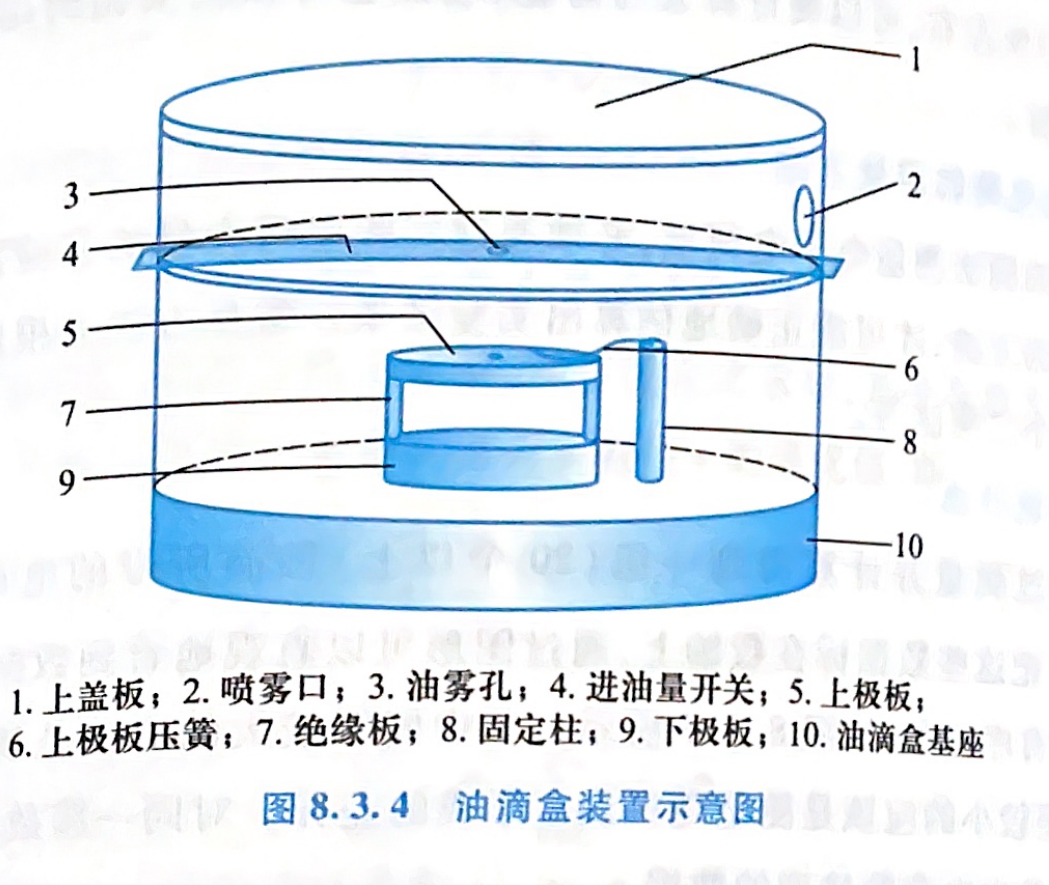
\includegraphics[width=7.2cm]{figures/millikan-chamber.png}\par
{\small 油滴盒结构示意图。}\end{center}
\ReportSection{实验内容}
\ReportSubsection{观测准备}
1. 检查油滴盒清洁、照明、显微镜调焦和极板电压零点；喷入少量油雾，选取孤立且运动缓慢的油滴。\par
2. 标定目镜中的固定下降距离。关闭电场，待油滴运动稳定后计时；同一滴重复四次，若轨迹偏离或油滴消失，应重新选滴。\par
\ReportSubsection{平衡与重复测量}
3. 逐渐增大电压，使油滴尽可能悬浮，记录平衡电压。对多颗油滴重复下降计时与电压测量。\par
4. 分别计算 $q_i$、整数 $n_i$ 和 $\frac{q_i}{n_i}$；绘制散点与拟合直线，比较反向验证值、图解斜率和最小二乘结果。
\ReportSection{实验仪器}
密立根油滴仪（油滴盒、电极板、照明及显微镜）、喷油器、计时器和直流高压电源。极板间距、空气黏度与修正常数已包含在仪器给定的计算常数中。
\ReportSection{数据记录处理}
\ReportSubsection{实验数据表}
\begin{center}\small\renewcommand{\arraystretch}{1.28}
\begin{adjustbox}{max width=\textwidth}
\begin{tabular}{|c|c|c|c|c|c|c|c|c|c|}\hline
测量次数 $i$ & 电压 $U$/V & $t_1$/s & $t_2$/s & $t_3$/s & $t_4$/s & $\bar t$/s & $q_i/10^{-19}$ C & 取整 $n_i$ & $e_i/10^{-19}$ C\\\hline
1 & \Field[7mm]{voltage_01} & \Field[7mm]{time_01_1} & \Field[7mm]{time_01_2} & \Field[7mm]{time_01_3} & \Field[7mm]{time_01_4} & \Field[7mm]{time_mean_01} & \Field[7mm]{charge_scaled_01} & \Field[7mm]{electron_count_01} & \Field[7mm]{charge_per_e_01}\\\hline
2 & \Field[7mm]{voltage_02} & \Field[7mm]{time_02_1} & \Field[7mm]{time_02_2} & \Field[7mm]{time_02_3} & \Field[7mm]{time_02_4} & \Field[7mm]{time_mean_02} & \Field[7mm]{charge_scaled_02} & \Field[7mm]{electron_count_02} & \Field[7mm]{charge_per_e_02}\\\hline
3 & \Field[7mm]{voltage_03} & \Field[7mm]{time_03_1} & \Field[7mm]{time_03_2} & \Field[7mm]{time_03_3} & \Field[7mm]{time_03_4} & \Field[7mm]{time_mean_03} & \Field[7mm]{charge_scaled_03} & \Field[7mm]{electron_count_03} & \Field[7mm]{charge_per_e_03}\\\hline
4 & \Field[7mm]{voltage_04} & \Field[7mm]{time_04_1} & \Field[7mm]{time_04_2} & \Field[7mm]{time_04_3} & \Field[7mm]{time_04_4} & \Field[7mm]{time_mean_04} & \Field[7mm]{charge_scaled_04} & \Field[7mm]{electron_count_04} & \Field[7mm]{charge_per_e_04}\\\hline
5 & \Field[7mm]{voltage_05} & \Field[7mm]{time_05_1} & \Field[7mm]{time_05_2} & \Field[7mm]{time_05_3} & \Field[7mm]{time_05_4} & \Field[7mm]{time_mean_05} & \Field[7mm]{charge_scaled_05} & \Field[7mm]{electron_count_05} & \Field[7mm]{charge_per_e_05}\\\hline
6 & \Field[7mm]{voltage_06} & \Field[7mm]{time_06_1} & \Field[7mm]{time_06_2} & \Field[7mm]{time_06_3} & \Field[7mm]{time_06_4} & \Field[7mm]{time_mean_06} & \Field[7mm]{charge_scaled_06} & \Field[7mm]{electron_count_06} & \Field[7mm]{charge_per_e_06}\\\hline
7 & \Field[7mm]{voltage_07} & \Field[7mm]{time_07_1} & \Field[7mm]{time_07_2} & \Field[7mm]{time_07_3} & \Field[7mm]{time_07_4} & \Field[7mm]{time_mean_07} & \Field[7mm]{charge_scaled_07} & \Field[7mm]{electron_count_07} & \Field[7mm]{charge_per_e_07}\\\hline
8 & \Field[7mm]{voltage_08} & \Field[7mm]{time_08_1} & \Field[7mm]{time_08_2} & \Field[7mm]{time_08_3} & \Field[7mm]{time_08_4} & \Field[7mm]{time_mean_08} & \Field[7mm]{charge_scaled_08} & \Field[7mm]{electron_count_08} & \Field[7mm]{charge_per_e_08}\\\hline
9 & \Field[7mm]{voltage_09} & \Field[7mm]{time_09_1} & \Field[7mm]{time_09_2} & \Field[7mm]{time_09_3} & \Field[7mm]{time_09_4} & \Field[7mm]{time_mean_09} & \Field[7mm]{charge_scaled_09} & \Field[7mm]{electron_count_09} & \Field[7mm]{charge_per_e_09}\\\hline
10 & \Field[7mm]{voltage_10} & \Field[7mm]{time_10_1} & \Field[7mm]{time_10_2} & \Field[7mm]{time_10_3} & \Field[7mm]{time_10_4} & \Field[7mm]{time_mean_10} & \Field[7mm]{charge_scaled_10} & \Field[7mm]{electron_count_10} & \Field[7mm]{charge_per_e_10}\\\hline
\end{tabular}
\end{adjustbox}\end{center}
\ReportSubsection{方法一：反向验证法}
\noindent 每滴 $e_i=q_i/n_i$。电子电荷量平均值
$\bar e=\MathField{electron_charge_reverse}\,\mathrm C$；
不确定度 $u_e=\MathField{electron_charge_reverse_u}\,\mathrm C$；
与公认值的百分差 $E=\Field{reverse_error_percent}\%$。
\ReportSubsection{方法二：图解法}
\noindent 作 $q_i$—$n_i$ 图，直线斜率对应电子电荷量：
$e=(\MathField{electron_charge_graph}\pm\MathField{electron_charge_graph_u})\,\mathrm C$。
\ReportSubsection{方法三：最小二乘法}
\noindent 过原点拟合 $e=\dfrac{\sum_i n_iq_i}{\sum_i n_i^2}$，
最优值 $e=\MathField{electron_charge_ls}\,\mathrm C$；
不确定度 $u_e=\MathField{electron_charge_ls_u}\,\mathrm C$；
百分差 $E=\Field{ls_error_percent}\%$。
\ReportSection{图解法：电荷量与整数倍数}
以 $n_i$ 为横轴、$\frac{q_i}{10^{-19}\,\mathrm C}$ 为纵轴，将已上传油滴的计算值逐点绘出。直线为带截距的线性拟合 $q=en+b$，其斜率对应图解法元电荷估计；该曲线由本次输入的电压和下降时间实时计算。
\begin{center}\begin{tikzpicture}
\begin{axis}[width=.88\textwidth,height=7cm,xlabel={$n_i$},ylabel={$\frac{q_i}{10^{-19}\,\mathrm C}$},grid=both,legend pos=north west]
\addplot+[only marks,mark=*,mark size=2pt] coordinates {\PlotCoordinates{charge_graph_points}};
\addlegendentry{油滴数据}
\addplot+[no marks,thick,blue] coordinates {\PlotCoordinates{charge_graph_fit_points}};
\addlegendentry{线性拟合}
\end{axis}\end{tikzpicture}\par
{\small 图解斜率 $e=(\MathField{electron_charge_graph}\pm\MathField{electron_charge_graph_u})\,\mathrm C$，截距 $b=\MathField{electron_charge_graph_intercept}\,\mathrm C$。}
\end{center}
\ReportSection{讨论与分析}
\ReportSubsection{图形与数值的对照}
图中每个散点都来自一颗油滴的四次平均下降时间与平衡电压。若某点明显偏离拟合线，应回查该滴是否发生蒸发、带电量跳变或布朗运动；不应只为得到整齐直线而删去读数。图解法允许非零截距，过原点最小二乘法则强制符合 $q=ne$，两种斜率的差异可以反映系统偏差。\par
\ReportSubsection{主要误差与改进}
下降时间过短会放大按表计时的相对误差；平衡状态的人工判断、极板电压波动、空气流动及焦平面变化也影响结果。选取运动较慢且稳定的油滴，保持油滴盒清洁并多次计时，可减小这些影响。\par
\ReportSubsection{思考题}
为何测量多颗油滴？单颗油滴只能给出一个电荷估计，无法可靠检验整数倍规律。为何先记录自由下降时间再调节平衡电压？下降速度用于估计油滴尺寸和有效重力，平衡电压再确定所带电荷量。
\ReportSection{实验结论}
本次实验以多颗油滴检验电荷量子化。反向验证得到 $e_{\rm rev}=(\MathField{electron_charge_reverse}\pm\MathField{electron_charge_reverse_u})\,\mathrm C$，图解拟合斜率为 $e_{\rm graph}=(\MathField{electron_charge_graph}\pm\MathField{electron_charge_graph_u})\,\mathrm C$，过原点最小二乘结果为 $e_{\rm ls}=(\MathField{electron_charge_ls}\pm\MathField{electron_charge_ls_u})\,\mathrm C$。三种结果应结合散点分布与不确定度比较。

\ReportRecord
% ===== 原始数据图片插入区 =====
\end{document}
